% ---------------------------------------------------------------------------------------------------------------------
% Evidence-first customer support triage: evaluation on Docker support.
% Prepared for the IEEE conference template (class `ieeeconf`, see conference_format.pdf).
%   * Put the template's ieeeconf.cls and IEEEtran.bst next to this file (the template is the only accepted format).
%   * Replace the author block below with the one from the template's own sample main.tex if its commands differ.
%   * Review versions: use [singleanonymous] or [doubleanonymous] instead of [cameraready].
%   * Build: pdflatex main; bibtex main; pdflatex main; pdflatex main
% ---------------------------------------------------------------------------------------------------------------------
\documentclass[cameraready]{ieeeconf}

\usepackage{graphicx}
\usepackage{booktabs}
\usepackage{amsmath}

\title{Evidence-First Customer Support Triage with Clarifying Questions, Gated Retrieval and Escalation: An Evaluation on Docker Support}

% TODO: replace with the real authors and affiliations (names italic, affiliations upright, as in the template's sample).
\author{Author A$^{1}$, Author B$^{1}$, Author C$^{1}$ \\
$^{1}$Affiliation, Address of Affiliation}

\begin{document}
\maketitle

\begin{abstract}
Support teams want automated answers that are grounded in documentation, but a wrong fix costs more than a hand-over to an engineer.
We describe an evidence-first triage agent for Docker support. A rule-based Clarifier asks at most three questions. A Resolver then checks a cache of confirmed answers, retrieves documentation with hybrid dense and keyword search and a small knowledge graph, applies a confidence gate, drafts a cited fix with a language model, verifies every step with rules, and escalates to a person when the evidence is weak.
We evaluate the system end to end with real Gemini calls, a simulated customer and an oracle, on 89 real and written support questions, 40 customer paraphrases of documented issues and 29 hand-written scenarios, with and without the knowledge graph.
The agent is safe: all 70 questions that should not get an automated fix were handed to a person or declined, and one or two of 89 received a wrong fix. It automates little on real questions, though: only 2--4 of 19 answerable real questions received a correct first fix, against 85--90\% on the hand-written scenarios. For 11 of the 15 escalated answerable questions the right page had been retrieved and the confidence gate declined to answer. The knowledge graph helped in direction but no difference was significant. We also report cache behaviour, a cache defect found and fixed, latency, cost and faithfulness, and the limits of the evidence.
\end{abstract}

\section{Introduction}
Technical support teams answer the same kinds of question again and again, and most answers already exist in public documentation. Large language models (LLMs) can turn documentation into fluent step-by-step fixes, but a fluent wrong fix is worse than a hand-over to an engineer. A support agent therefore has to decide three things for every message: whether it understands the problem well enough, whether the evidence it found is good enough to answer, and whether to escalate. Retrieval-augmented generation (RAG) \cite{lewis2020rag} grounds an answer in retrieved text, but retrieval alone does not say whether the retrieved text is good enough.

We built and evaluated an evidence-first triage agent for Docker support around three rules: every step of a fix must be traceable to retrieved documentation; weak evidence leads to escalation, not a guess; and a language model is used for as few steps as possible, so that most of the system is inspectable rules and search.

This paper makes four contributions.
\begin{itemize}
\item A two-agent architecture: a rule-based Clarifier that asks at most three questions, and a Resolver with a cache, hybrid retrieval with a small knowledge graph, a confidence gate, drafting, a rule-based verifier and escalation (Section~\ref{sec:design}).
\item An evaluation harness with a simulated customer, an oracle, feature-flagged ablation arms that run side by side, retries and run-validity checks, and per-query logs (Section~\ref{sec:setup}).
\item Real-model results on three test sets with nine metrics (Section~\ref{sec:results}).
\item An analysis of where answerable questions are lost, of what the knowledge graph does and does not change, and of a cache defect found and fixed during the evaluation (Sections~\ref{sec:results} and~\ref{sec:discussion}).
\end{itemize}

The headline result is a gap between safety and coverage. The agent handed over or declined every question that should not get an automated fix, yet gave a correct first fix for only 2 to 4 of 19 answerable real questions. The main loss is the confidence gate, not retrieval: it declined to answer when the right page was already among the results.

\section{Related work}
\textbf{Retrieval and fusion.} RAG \cite{lewis2020rag} conditions generation on retrieved passages. We combine keyword search with BM25 \cite{robertson2009bm25}, dense retrieval with the BGE embedding family \cite{xiao2023cpack}, and reciprocal rank fusion \cite{cormack2009rrf}.

\textbf{Customer-support RAG.} Xu et al.\ \cite{xu2024kgrag} build a knowledge graph from historical support tickets and report a 77.6\% MRR improvement and a 28.6\% cut in median resolution time after deployment. We instead use curated documentation and a small hand-built ontology, and we measure end-to-end behaviour, not retrieval alone. Rakin et al.\ \cite{rakin2024domain} adapt RAG models to hotel customer service to reduce hallucination.

\textbf{Agent evaluation.} $\tau$-bench \cite{yao2024taubench} evaluates agents against a simulated user and compares the final state with a goal; we adopt the simulated customer and an oracle that checks the final answer. CirrusBench \cite{yu2026cirrusbench} argues for measuring resolution efficiency beyond correctness, which motivates our question, latency and cost metrics.

\textbf{Escalation and consistency.} Montgomery et al.\ \cite{montgomery2020escalation} predict which tickets will escalate from ticket features. We decide at answer time, from the strength of the evidence. Zimmerman et al.\ \cite{zimmerman2024hallucination} detect LLM answers that are inconsistent with a knowledge base using encoder models; we verify each step by rules and use an LLM judge only for evaluation.

\textbf{Caching and reranking.} Regmi and Pun \cite{regmi2024semcache} cache answers by embedding similarity and report hit rates of 61.6--68.8\%. We cache only answers a customer confirmed, and evict an entry when a customer rejects its answer. Tiwari and Kumar \cite{tiwari2026shopease} found that adding a cross-encoder reranker raised latency without improving accuracy; our reranking is switched off.

\section{System design}\label{sec:design}
\subsection{Overview}
A customer describes a problem in free text and may attach a screenshot, which is read with optical character recognition. Fig.~\ref{fig:pipeline} shows the path of one case. Rules first strip greetings and pasted log noise, reject prompt injection and requests for secrets, and send data-loss and security cases straight to a person. A scope check by an LLM runs only when the message has no clear Docker wording; it can only decline, and only when at least 80\% sure, and a failed call lets the question through.

\begin{figure*}[t]
\centering
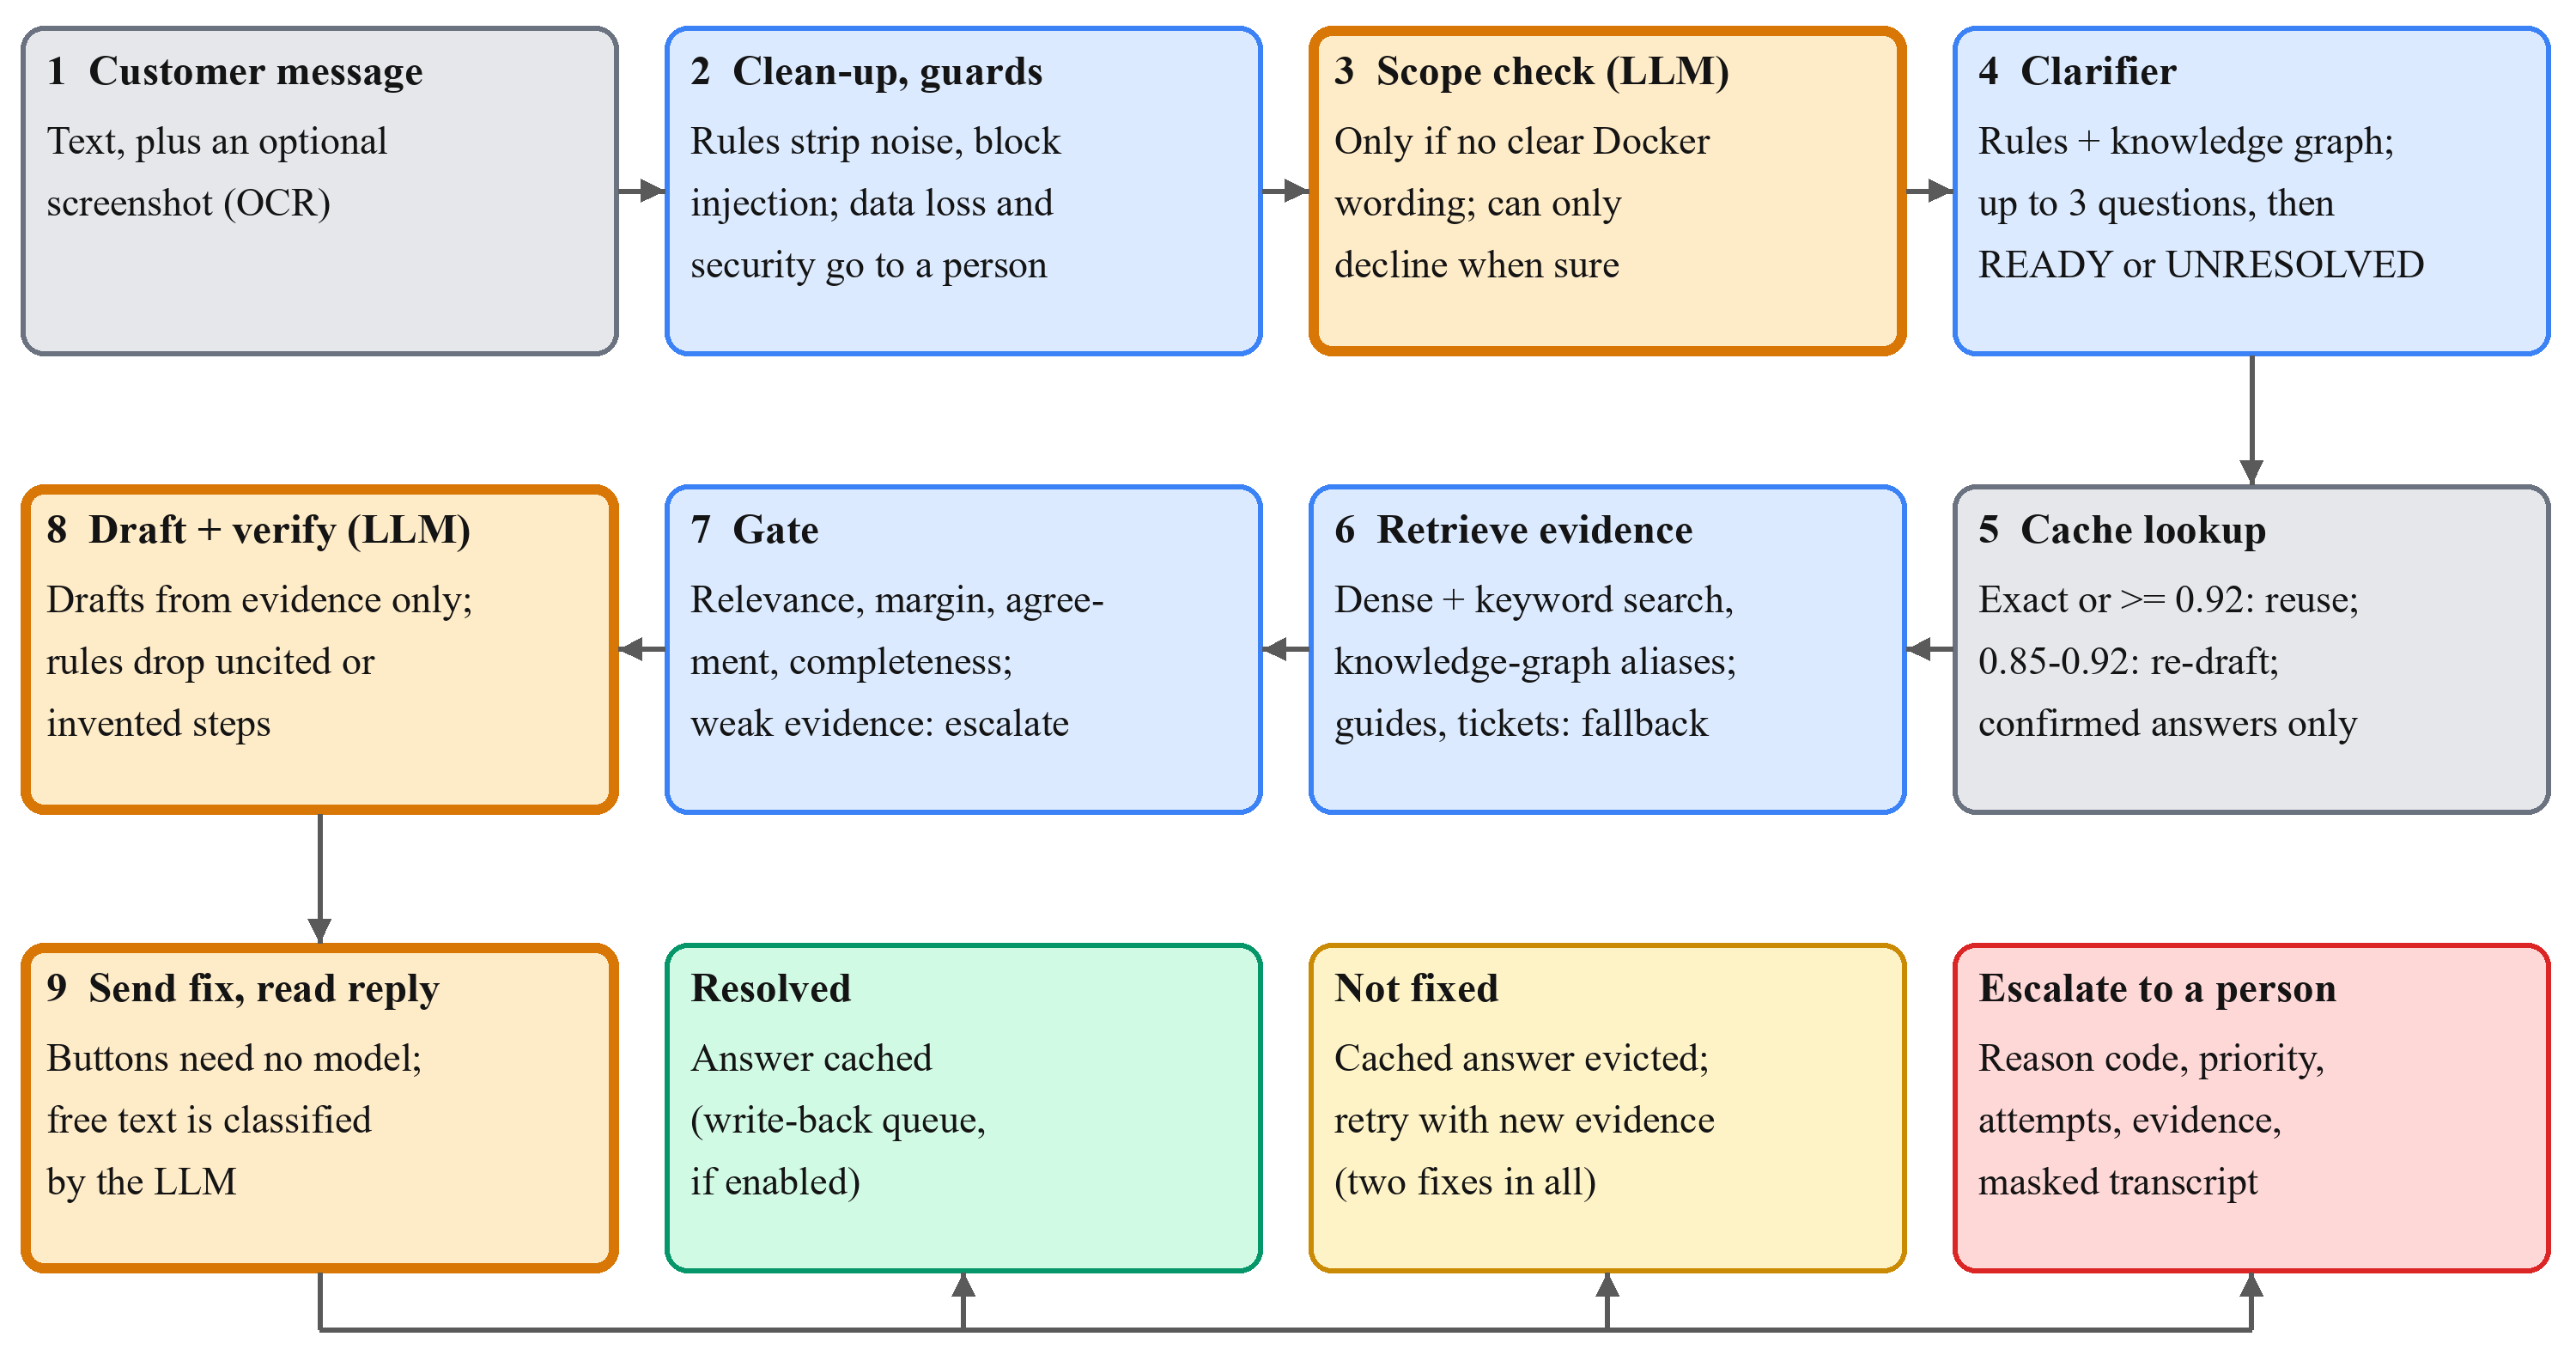
\includegraphics[width=\textwidth]{figures/pipeline_colour.png}
\caption{Path of one case. Blue boxes use rules only; orange boxes with a bold outline call the language model; grey boxes are input or storage; green, amber and red boxes are outcomes. New information in a reply returns the case to the Clarifier.}
\label{fig:pipeline}
\end{figure*}

Only three steps call the LLM: the scope check, drafting, and classifying a free-text reply. Everything else is rules and search, so a case that is escalated before drafting makes no model call.

\subsection{Clarifier}
The Clarifier uses no model. Rules extract the platform, product area, error and exit codes and versions from the message, assisted by the knowledge graph. It searches the documentation and turns the scores into a probability over candidate issues with a softmax (temperature 0.08). It reports READY when the leading issue holds at least half the probability and leads the runner-up by at least 0.25. Otherwise it asks the question that best separates the leading candidates, at most three times; a case it cannot pin down is UNRESOLVED.

\subsection{Knowledge sources and retrieval}
The main evidence is the public Docker documentation \cite{dockerdocs}: 961 pages split into 11,440 passages. Two smaller sources are consulted only on a fallback path. A small tier of third-party guides is searched when the best official relevance is below 0.55, and its scores are weighted by 0.85. Resolved community tickets (13,092 indexed) are used only when the Clarifier was READY but the documentation was weak, and are always labelled as community answers.

A query is searched with dense retrieval (BAAI/bge-base-en-v1.5) and BM25 over headings and text, taking 30 results from each. The two rankings are merged with reciprocal rank fusion with equal weights,
\begin{equation}
\mathrm{RRF}(d)=\sum_{r\in\{\mathrm{dense},\,\mathrm{keyword}\}}\frac{1}{60+\operatorname{rank}_r(d)},
\label{eq:rrf}
\end{equation}
and the results are grouped into one evidence item per documented issue; the top 8 are returned. Each item carries a relevance score on an absolute scale from 0 to 1: the dense similarity, times a page-type weight, times $0.5+0.5\,\mathrm{coverage}$, where coverage is the share of the customer's words found in the issue.

The \emph{knowledge graph} holds 153 Docker entities (products, features, error names) with aliases, symptoms and error strings. When enabled, it adds alias terms to the keyword query, adds a third ranking of passages that share the entities found in the message, and lets the Clarifier name entities and infer the platform. Its 51 issue nodes link to documentation issues, which is 22\% of the 233 troubleshooting and FAQ issues (none of the 96 FAQ issues).

\subsection{Confidence gate}
Let $t$ be the relevance of the top evidence item, $m$ its margin over the second item, $a$ the agreement among the top items (raised to the Clarifier's probability for its leading issue when that is higher), and $q$ the completeness of the problem description. The gate computes
\begin{equation}
c = 0.45\,t + 0.15\,\min\!\left(\tfrac{m}{0.2},\,1\right) + 0.20\,a + 0.20\,q ,
\label{eq:gate}
\end{equation}
and answers only when $t\ge 0.55$, $c\ge 0.6$, and it is not the case that both $m<0.05$ and $a<0.4$. Otherwise it falls back to tickets or escalates. These thresholds are starting values chosen by hand; a calibration on an earlier, smaller sample left them unchanged.

\subsection{Drafting and verification}
The LLM (Gemini) is asked to write a fix using only the supplied evidence and to cite an evidence identifier for each step. Rules then drop any step whose citation is missing or invalid, or whose command or link does not occur in the cited text, and reject the draft when fewer than half the steps survive. The customer's reply is classified as resolved, not fixed, new information or off topic (chat buttons need no model). A rejected fix is retried once with new evidence, so at most two fixes are sent, and then the case escalates.

\subsection{Semantic cache}
The cache stores answers that a customer confirmed. A lookup first tries an exact match on the problem signature. Otherwise an entry is considered only if its product, component, error text and leading issue agree; a similarity of at least 0.92 reuses the answer, and 0.85 to 0.92 reuses the evidence and drafts again. During the evaluation we found that a rejected cached answer was served again to the next similar customer, so a rejection now switches that entry off. Entries also expire when their source documents change.

\subsection{Escalation}
An escalated case carries a reason code (for example low evidence, retry exhausted, verification failed, out of scope, security or data loss), a priority, the attempts, the evidence, and a transcript with personal data masked.

\section{Experimental setup}\label{sec:setup}
\subsection{Test sets}
\textbf{Real questions (89).} Real questions plus guard cases: 19 answerable questions (the documentation has the fix), 46 real questions the documentation cannot answer, 8 vague, 6 urgent, 6 not about Docker and 4 prompt-injection attempts. Sixty-five are real Stack Overflow questions; the other 24 were written as regression guards. Eight of the 19 answerable labels are weaker than the rest. \textbf{Paraphrases (40).} Customer wordings of documented issues, written to test whether the knowledge graph helps when the customer's words differ from the documentation's; two of the original 42 accept two answers and are left out. All 40 documented issues have a graph node. \textbf{Scenarios (29).} Hand-written cases, 20 with a documented answer and 9 without, each asked once and then 9 of them asked again word for word.

\subsection{Arms}
Arm A has the knowledge graph switched off in retrieval and in the Clarifier; arm B has it on. Everything else is identical: the cache, the ticket fallback, the guides, the gate and the model. A third switch for a Jev-style decision layer exists in the code, but no step calls it, so it is not evaluated here.

\subsection{Simulated customer and oracle}
A rule-based customer answers the Clarifier's questions from hidden facts; for the real questions and paraphrases the only hidden fact is the wording itself, so questions are answered ``I'm not sure''. After each fix an oracle replies that it worked only when the fix cites the gold documentation issue, and ``still the same error'' otherwise. A fix drawn from community tickets is always rejected, because tickets have no gold label.

\subsection{Protocol}
All Gemini calls used gemini-3.5-flash-lite. The runs used the same committed code (commit 598a894, and daa7b2f for the paraphrases, which adds only the paraphrase converter), no uncommitted changes, and a fixed hash seed because the Clarifier breaks ties by hash order. The two arms advanced together, one question at a time, taking turns to go first, so that slow stretches of the model API are shared. Requests were paced to 15 per minute and a failed call was retried; a run is marked invalid if any call still fails, and none did. The knowledge-graph comparisons on real questions and paraphrases use the cache off, so that one case cannot affect another; the scenario run and a second real-question run use the cache on, with 30\% of questions asked again. All numbers come from the saved run logs (one per-question log and one summary per run) at the commits named above.

\subsection{Metrics}
We report nine metrics: (1) first-attempt correct, the share of answerable questions whose first fix cites the gold issue; (2) wrong-fix rate, over all questions and over answerable ones; (3) escalation recall, the share of questions that should not get an automated fix (no documented answer, vague, urgent, not about Docker, injection) that were handed to a person or declined; (4) escalation precision and the unnecessary-escalation rate; (5) Recall@3 and mean reciprocal rank (MRR) of the gold issue in the first search; (6) questions asked per case; (7) time to first fix; (8) citation validity; and (9) retrieval time and latency. Cache hit rate, precision and false-hit rate, cost and tokens come from the event log. Rates carry 95\% Wilson intervals \cite{wilson1927interval}, and paired differences are tested with an exact McNemar test.

\section{Results}\label{sec:results}
\begin{table*}[t]
\caption{Results for arm A (no knowledge graph) and arm B (with it). Rates are percentages with counts. Real questions: cache off. Scenarios: cache on, quality metrics on the first ask. The paraphrase set has no unanswerable question, so escalation recall and precision are undefined.}
\label{tab:main}
\centering
\footnotesize
\setlength{\tabcolsep}{4.5pt}
\begin{tabular}{@{}lrrrrrr@{}}
\toprule
 & \multicolumn{2}{c}{Real questions (89)} & \multicolumn{2}{c}{Paraphrases (40)} & \multicolumn{2}{c}{Scenarios (29 + 9 repeats)} \\
\cmidrule(lr){2-3}\cmidrule(lr){4-5}\cmidrule(lr){6-7}
Metric & A & B & A & B & A & B \\
\midrule
First-attempt correct (\%) & 10.5 (2/19) & 21.1 (4/19) & 57.5 (23/40) & 60.0 (24/40) & 85.0 (17/20) & 90.0 (18/20) \\
Wrong-fix rate, all questions (\%) & 2.2 (2/89) & 1.1 (1/89) & 5.0 (2/40) & 5.0 (2/40) & 6.9 (2/29) & 3.4 (1/29) \\
Wrong first fix, answerable (\%) & 10.5 (2/19) & 0.0 (0/19) & 5.0 (2/40) & 5.0 (2/40) & 5.0 (1/20) & 5.0 (1/20) \\
Escalation recall (\%) & 100.0 (70/70) & 100.0 (70/70) & -- & -- & 100.0 (9/9) & 100.0 (9/9) \\
Escalation precision (\%) & 80.5 (70/87) & 82.4 (70/85) & -- & -- & 81.8 (9/11) & 81.8 (9/11) \\
Unnecessary escalation (\%) & 89.5 (17/19) & 78.9 (15/19) & 40.0 (16/40) & 37.5 (15/40) & 10.0 (2/20) & 10.0 (2/20) \\
Recall@3 (\%) & 52.6 (10/19) & 63.2 (12/19) & 85.0 (34/40) & 90.0 (36/40) & 94.4 (17/18) & 94.4 (17/18) \\
MRR & 0.393 & 0.393 & 0.771 & 0.798 & 0.944 & 0.944 \\
Questions per case & 1.75 & 1.69 & 1.60 & 1.40 & 1.38 & 1.24 \\
Time to first fix p50/p95 (s) & 4.7/8.8 & 4.7/5.8 & 4.3/7.6 & 5.3/8.1 & 5.9/12.4 & 5.6/32.4 \\
Citation validity (\%) & 100.0 (4/4) & 100.0 (5/5) & 100.0 (27/27) & 100.0 (28/28) & 100.0 (19/19) & 100.0 (17/17) \\
Retrieval time p50 (ms) & 844 & 891 & 356 & 458 & 347 & 388 \\
End-to-end p50/p95 (s) & 2.3/7.0 & 2.3/7.2 & 5.6/15.6 & 6.9/15.3 & 6.9/15.9 & 6.5/19.1 \\
\midrule
Model calls & 22 & 27 & 72 & 76 & 65 & 60 \\
Input tokens (thousands) & 20.7 & 36.5 & 97.5 & 106.7 & 81.0 & 70.9 \\
Cost (USD) & 0.0103 & 0.0154 & 0.0448 & 0.0492 & 0.0374 & 0.0326 \\
\bottomrule
\end{tabular}
\end{table*}


\subsection{Real questions}
Table~\ref{tab:main} gives the results. Escalation recall (hand-over or refusal) is 70 of 70 in both arms (95\% interval 94.8--100\%), and every urgent, out-of-scope and injection question is handled correctly (Table~\ref{tab:classes}). A documentation fix is wrong for 2 of 89 questions in arm A and 1 of 89 in arm B.

\begin{figure*}[t]
\centering
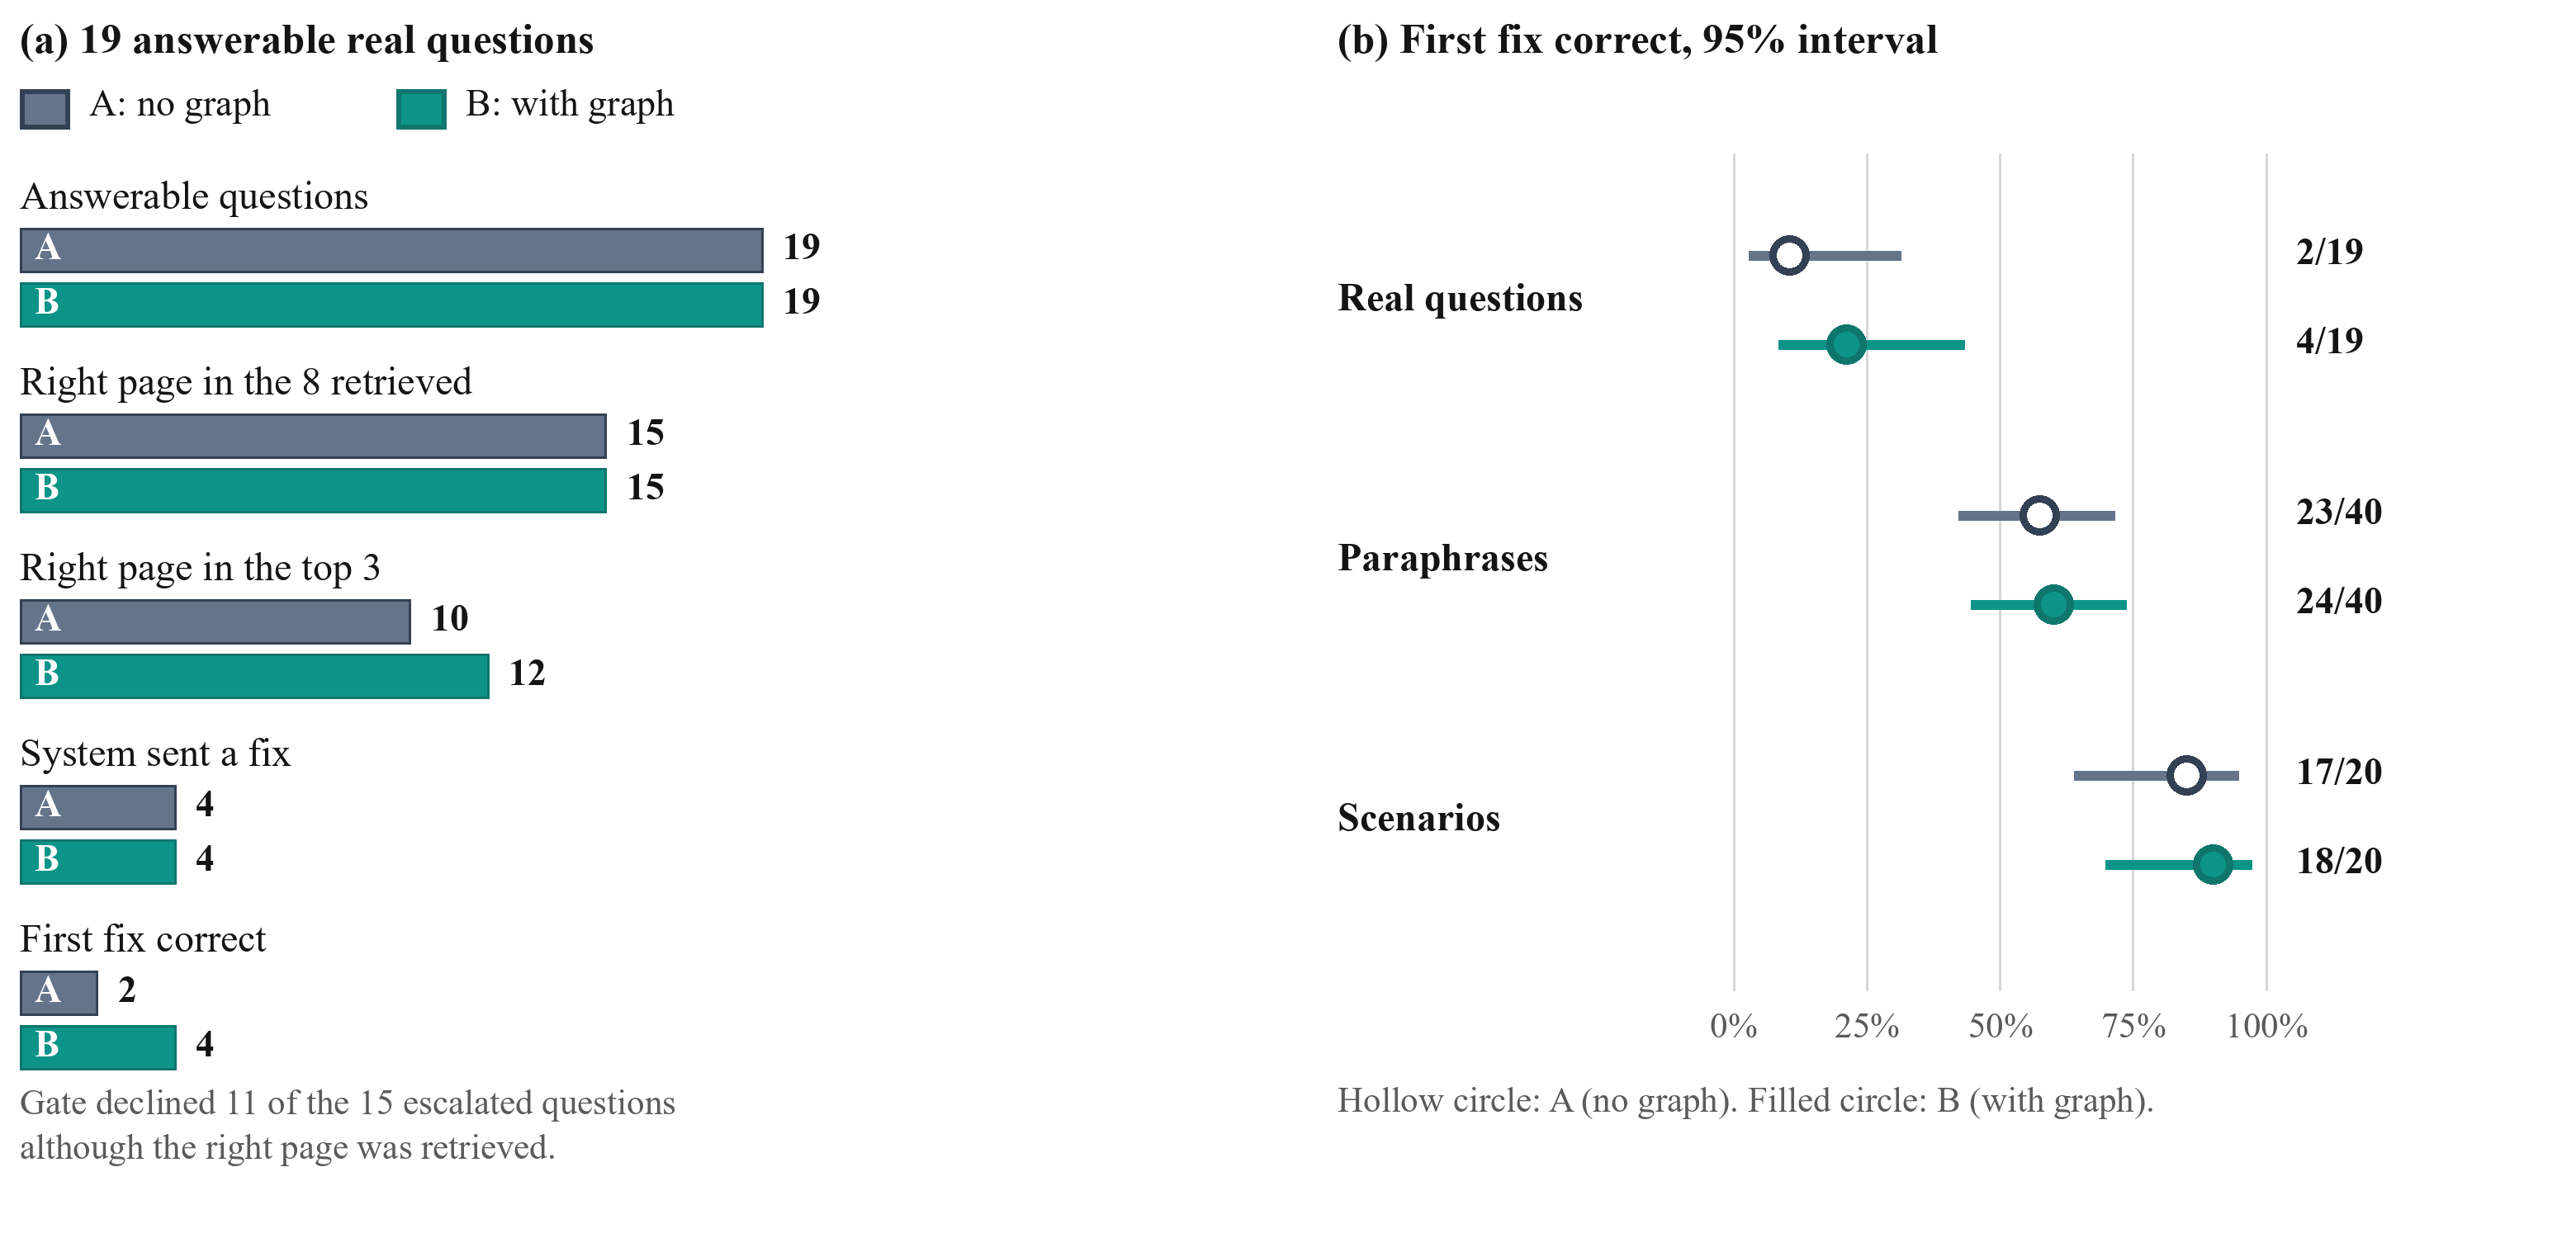
\includegraphics[width=\textwidth]{figures/results_colour.png}
\caption{(a) What happens to the 19 answerable real questions in each arm (grey-blue: arm A, no graph; teal: arm B, with graph). (b) First fix correct with 95\% Wilson intervals on the three test sets (hollow circle: A; filled circle: B).}
\label{fig:results}
\end{figure*}

The agent automates little. Only 2 of 19 answerable real questions (10.5\%, interval 2.9--31.4\%) receive a correct first fix in arm A and 4 (21.1\%, 8.5--43.3\%) in arm B, and 17 and 15 of 19 are escalated although the documentation has the answer. On the hand-written scenarios the same code scores 85--90\% (Fig.~\ref{fig:results}b).

\begin{table}[t]
\caption{Questions handled correctly by type (real questions, cache off). Correct means a right fix for answerable questions and a hand-over or refusal with no documentation fix for the rest.}
\label{tab:classes}
\centering
\footnotesize
\begin{tabular}{@{}lrrr@{}}
\toprule
Question type & $n$ & A & B \\
\midrule
Answerable & 19 & 2 & 4 \\
No documented answer & 46 & 46 & 45 \\
Vague & 8 & 7 & 7 \\
Urgent & 6 & 6 & 6 \\
Not about Docker & 6 & 6 & 6 \\
Prompt injection & 4 & 4 & 4 \\
\bottomrule
\end{tabular}
\end{table}


\subsection{Where answerable questions are lost}
Fig.~\ref{fig:results}a follows the 19 answerable questions. The right page is among the 8 retrieved issues for 15, and in the top 3 for 10 (arm A) or 12 (arm B). Only 4 questions end in a fix in either arm. Fifteen questions in each arm end without any fix, every one through a low-evidence decision by the gate (arm A also escalates two more after a wrong fix). For 11 of those 15 the right page was retrieved, at ranks 1 to 8, but the gate declined to answer: the right page's relevance was roughly 0.35 to 0.65, against a bar of 0.55 for the top result, and the right page was the top result for only 4 of the 19 questions. Four questions (H004, H014, H030, H034) are true retrieval misses. The gate is therefore the larger loss.

\subsection{Effect of the knowledge graph}
On real questions the graph finds a named Docker entity or alias in 45 of 89 questions (14 of 19 answerable), yet none of the 19 answerable questions has a graph node linked to its documented issue, so the graph's strongest function, mapping a symptom to a known issue, is not exercised. Arm B was better on H009 and H046 (escalated in A, answered correctly in B), and sent no wrong first fix where A sent two (H043 and H051, both through the ticket fallback), but it sent documentation fixes on questions with no documented answer (H047, and H037 with the cache on).

The paraphrases are built for the graph: it fires on 38 of 40, and all 40 have a linked node. Even so, first-attempt correct rises only from 23 to 24 of 40 (57.5\% to 60.0\%). The right page is in the top 8 for 34 questions in arm A and 37 in arm B, and Recall@3 rises from 85.0\% to 90.0\% (MRR 0.771 to 0.798). Arm B was better on P08, P19 and P33 and worse on P22 and P41, and it sent a wrong fix on P14 where A escalated while A sent one on P23 where B escalated. Of the escalated questions, 9 of 15 (A) and 11 of 14 (B) had the right page retrieved.

On the scenarios the arms differ in first-attempt correctness on one question (S10). No paired difference is significant (exact McNemar $p=0.5$ on real questions, $p=1$ on paraphrases and scenarios). An earlier retrieval-only run on the 42 original paraphrases reported Recall@8 rising from 0.833 to 0.976 with the graph, so the graph improves retrieval more than it improves answers: the gate absorbs much of the gain.

\subsection{Cache}
\begin{table}[t]
\caption{Semantic cache with the cache on, as counts. A hit is an answer served from the cache; a false hit is a hit whose first fix was not correct.}
\label{tab:cache}
\centering
\footnotesize
\setlength{\tabcolsep}{3pt}
\begin{tabular}{@{}lrrrr@{}}
\toprule
 & \multicolumn{2}{c}{Scenarios} & \multicolumn{2}{c}{Real questions} \\
\cmidrule(lr){2-3}\cmidrule(lr){4-5}
 & A & B & A & B \\
\midrule
Hits / lookups & 6/33 & 7/33 & 1/82 & 1/82 \\
Correct / hits & 6/6 & 6/7 & 1/1 & 1/1 \\
False hits / hits & 0/6 & 1/7 & 0/1 & 0/1 \\
Repeat speed-up ($\times$) & 2.13 & 2.07 & 1.52 & 1.83 \\
\bottomrule
\end{tabular}
\end{table}

Table~\ref{tab:cache} shows the cache. On the scenarios the hit rate is 18.2\% in arm A and 21.2\% in arm B, including one semantic hit on a first ask (S03, answered from a similar earlier question), and all five repeated questions that had been resolved (S02, S09, S13, S14, S16) were answered from the cache in both arms, about 2.1 times faster end to end. One false hit remains in arm B: S17, a rootless-pull question, matched an unrelated ``Docker daemon not running'' answer at a similarity of 0.9237, just above the 0.92 threshold. In an earlier run on the same scenarios, before rejected answers were evicted, that wrong answer was served again when S17 was repeated (2 false hits of 8 in arm B); after the fix the repeat misses the cache. On real questions the hit rate is 1.2\% (1 of 82): of 27 repeated questions, 26 ended without a fix, and the cache stores only confirmed answers, so every repeat paid the full pipeline.

\subsection{Latency and cost}
With the arms interleaved, median end-to-end time on real questions is 2.3 s in both arms, because most cases end without drafting; it is 5.6 s (A) and 6.9 s (B) on paraphrases and 6.9 s and 6.5 s on scenarios. The graph adds 41 to 102 ms to the median retrieval call. A drafted case makes about two Gemini calls and costs about \$0.001. Arm B costs more on real questions and paraphrases because it answers more questions, and less on scenarios. The four runs cost about \$0.22 in total. The slow 95th percentile of arm B on scenarios (32 s) comes from one question that took 35 s after a retried call.

\subsection{Faithfulness}
A Gemini judge (the model that drafted the fixes, without planted-fault controls) split the 19 fixes sent by arm B on the scenarios into 90 claims. Mean claim support was 0.926 and all 19 fixes addressed the problem. Thirteen fixes were fully supported; six contained an unsupported claim, and in every case that claim was the closing confirmation step the reply template adds. All 73 other claims were supported, while the judge accepted the confirmation line in 11 of its 17 occurrences.

\section{Discussion}\label{sec:discussion}
\textbf{Safety is high; coverage on real questions is low.} Hand-over worked for every question that needed it, and wrong fixes were rare. But the agent resolved only 10--21\% of answerable real questions on the first attempt, so most of the saving a deployment hopes for is not realised. The 85--90\% on hand-written scenarios, and 57--60\% on paraphrases, show how much easier author-written questions are; they should not be used as headline numbers.

\textbf{The gate is the main lever.} For 11 of 15 escalated answerable questions the right page was retrieved. Loosening the gate would answer more of them but also more wrongly, so its thresholds need calibrating on real questions; an earlier calibration on a smaller sample kept them. Improving retrieval is the second lever: four questions are never retrieved.

\textbf{The knowledge graph points the right way, unproven.} It gave more correct first fixes in all three sets and removed two wrong first fixes on real questions, but every difference is one or two questions, all intervals overlap, and no test is significant. One real question flipped between two runs of the same arm, so a one-question gap is within run-to-run noise. The graph also cannot help most real questions, because it has a node for only 22\% of the documented issues.

\textbf{Threats to validity.} (i) Each setting was run once, and only 19 real questions are answerable. (ii) The customer is simulated by rules and the oracle accepts only the gold issue, so a correct fix from another page counts as wrong. (iii) Eight of the 19 answerable labels are weak, the 65 real questions were examined while the system was tuned, and the graph and the paraphrases share authors, which favours the graph. (iv) Repeats are word for word, so reworded repeats and the semantic hit rate are barely tested. (v) The judge shares the drafter's model and was not validated. (vi) Latency depends on a hosted model whose speed varies; interleaving the arms removes drift between them but not between runs. (vii) The planned Jev decision-layer arm was not implemented.

\section{Conclusion and future work}
We presented an evidence-first support agent and evaluated it end to end with a real model. It hands over what it cannot answer and rarely sends a wrong fix, but on real questions its confidence gate declines most answerable cases even when the right documentation was retrieved. The knowledge graph moves results in the right direction without a significant effect, and the evaluation exposed and fixed a cache defect.

Future work follows the findings. First, calibrate the gate on real questions and compare a tuned threshold with a learned decision layer over the gate's own inputs, such as a logistic classifier or a small decision model, which is the experiment our unused third switch was meant for. Second, grow and double-label the set of answerable questions, and repeat each setting to put run-to-run variation into the intervals. Third, extend the graph to the issues real questions are about, and test it with a development and a separate test split. Fourth, calibrate the cache threshold with more look-alike question pairs, and have people grade a sample of fixes.

\bibliographystyle{IEEEtran}
\bibliography{references}

\end{document}
